The HfO$_2$-based ferroelectric breakthrough enabled fast non-volatile operation with CMOS-friendly integration. 
FeFET cells (1T) drastically reduce footprint while offering in-class switching. 
Key challenges include polarization variability, fatigue, retention, and TDDB---especially under scaled dimensions.
Recent directions combine HfO$_2$ ferroelectrics with flexible substrates and explore radiation tolerance for extreme environments.

\begin{figure}[!t]
\centering
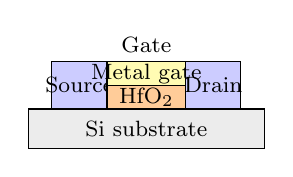
\begin{tikzpicture}[font=\footnotesize]

% 基板
\draw[fill=gray!15] (-1.5,0) rectangle (1.5,-0.5);
\node at (0,-0.25) {Si substrate};

% ソース・ドレイン
\draw[fill=blue!20] (-1.2,0) rectangle (-0.5,0.6);
\draw[fill=blue!20] (0.5,0) rectangle (1.2,0.6);
\node at (-0.85,0.3) {Source};
\node at (0.85,0.3) {Drain};

% ゲート stack
\draw[fill=orange!40] (-0.5,0) rectangle (0.5,0.3);
\node at (0,0.15) {HfO$_2$};

\draw[fill=yellow!30] (-0.5,0.3) rectangle (0.5,0.6);
\node at (0,0.45) {Metal gate};

% ゲートラベル
\node[above] at (0,0.6) {Gate};

\end{tikzpicture}
\caption{Schematic of a FeFET: HfO$_2$ ferroelectric layer integrated into the MOSFET gate stack.}
\label{fig:feram_fefet}
\end{figure}
